\documentclass[aspectratio=169]{beamer}

% ── Theme ──────────────────────────────────────────────────
\usetheme{metropolis}
\usepackage{booktabs}
\usepackage{amsmath}
\usepackage{graphicx}
\usepackage{tikz}

\definecolor{mDarkTeal}{HTML}{23373b}
\definecolor{mLightGreen}{HTML}{14B03D}

\title{Unsupervised Neural Machine Translation\\for Turkish--English}
\subtitle{CENG467 Term Project — Group 9}
\author{Ali Alp Haraç \& İhsan Yağız Sakızlıoğlu}
\date{June 2026}
\institute{Izmir Institute of Technology}

\begin{document}

% ══════════════════════════════════════════════════════════
%  TITLE
% ══════════════════════════════════════════════════════════
\begin{frame}
  \titlepage
\end{frame}

% ══════════════════════════════════════════════════════════
%  OUTLINE
% ══════════════════════════════════════════════════════════
\begin{frame}{Outline}
  \tableofcontents
\end{frame}

% ══════════════════════════════════════════════════════════
\section{Problem \& Motivation}
% ══════════════════════════════════════════════════════════

\begin{frame}{The Problem}
  \begin{itemize}
    \item State-of-the-art NMT requires \textbf{millions of parallel sentences}
    \item Parallel data is \textbf{scarce, expensive}, and unavailable for most language pairs
    \item \textbf{Question:} Can we train a translation system using \emph{only} monolingual data?
  \end{itemize}
  \vfill
  \begin{center}
    \Large $\underbrace{\text{1M Turkish sentences}}_{\text{No translations!}} + \underbrace{\text{1M English sentences}}_{\text{No translations!}} \xrightarrow{?} \text{Translator}$
  \end{center}
\end{frame}

\begin{frame}{Why Turkish--English?}
  \begin{itemize}
    \item \textbf{Morphologically rich:} Turkish is agglutinative \\
          \quad \textit{``yapamayacaklarımızdan''} = a single word with 5+ morphemes
    \item \textbf{Structurally different:} SOV vs.\ SVO word order
    \item Makes unsupervised alignment especially challenging
    \item Following the framework of \textbf{Lample et al.\ (2018)}
  \end{itemize}
\end{frame}

% ══════════════════════════════════════════════════════════
\section{Methodology}
% ══════════════════════════════════════════════════════════

\begin{frame}{System Overview}
  \begin{center}
    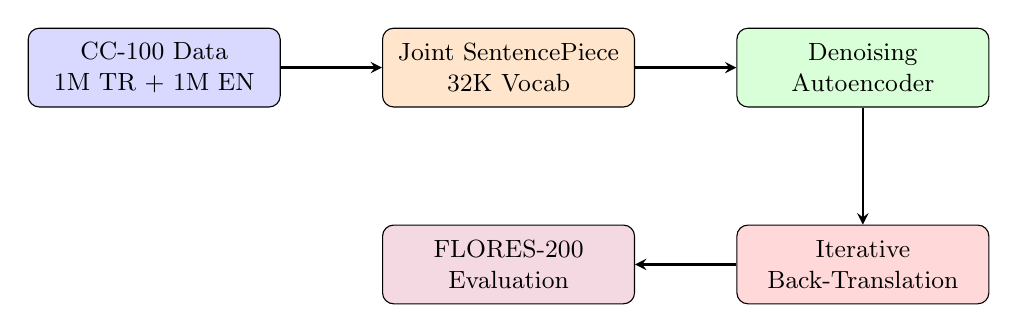
\begin{tikzpicture}[
      box/.style={draw, rounded corners, minimum width=3.2cm, minimum height=1cm, align=center, font=\small},
      arrow/.style={->, thick, >=stealth}
    ]
      \node[box, fill=blue!15] (data)   at (0,0)   {CC-100 Data\\1M TR + 1M EN};
      \node[box, fill=orange!20] (sp)   at (4.5,0) {Joint SentencePiece\\32K Vocab};
      \node[box, fill=green!15] (dae)   at (9,0)   {Denoising\\Autoencoder};
      \node[box, fill=red!15] (ibt)    at (9,-2.5) {Iterative\\Back-Translation};
      \node[box, fill=purple!15] (eval) at (4.5,-2.5) {FLORES-200\\Evaluation};
      
      \draw[arrow] (data) -- (sp);
      \draw[arrow] (sp) -- (dae);
      \draw[arrow] (dae) -- (ibt);
      \draw[arrow] (ibt) -- (eval);
    \end{tikzpicture}
  \end{center}
\end{frame}

\begin{frame}{Step 1: Shared Vocabulary}
  \begin{itemize}
    \item Joint \textbf{SentencePiece} (Unigram) model trained on both languages
    \item Vocabulary size: \textbf{32,000} subwords
    \item Creates a shared embedding space for Turkish and English
    \item Example: \textit{``yapamayacakları''} $\rightarrow$ \texttt{[\_yap, ama, yacak, ları]}
  \end{itemize}
\end{frame}

\begin{frame}{Step 2: Denoising Autoencoder (DAE)}
  \begin{columns}
    \column{0.55\textwidth}
    \begin{itemize}
      \item Corrupt input with three noise types:
      \begin{enumerate}
        \item \textbf{Word Shuffle} ($k=3$)
        \item \textbf{Word Dropout} ($p=0.1$)
        \item \textbf{Word Masking} ($p=0.1$)
      \end{enumerate}
      \item Model learns to \textbf{reconstruct} the original
      \item Learns grammar \& structure of \emph{both} languages
    \end{itemize}
    \column{0.4\textwidth}
    \begin{exampleblock}{Example}
      \textbf{Input:} ``The cat sat on the mat'' \\[4pt]
      \textbf{Noisy:} ``cat \texttt{<MASK>} the on sat'' \\[4pt]
      \textbf{Output:} ``The cat sat on the mat'' \\[4pt]
      $\rightarrow$ \textit{Model learns language!}
    \end{exampleblock}
  \end{columns}
\end{frame}

\begin{frame}{Step 3: Iterative Back-Translation (IBT)}
  \begin{columns}
    \column{0.55\textwidth}
    \begin{enumerate}
      \item Translate TR $\rightarrow$ EN (noisy, synthetic)
      \item Train model: synthetic EN $\rightarrow$ real TR
      \item Translate EN $\rightarrow$ TR (noisy, synthetic)
      \item Train model: synthetic TR $\rightarrow$ real EN
      \item \textbf{Repeat} — quality improves each iteration!
    \end{enumerate}
    \column{0.4\textwidth}
    \begin{alertblock}{Key Insight}
      The model uses its \emph{own mistakes} as training signal.
      Like learning a language by translating back and forth!
    \end{alertblock}
  \end{columns}
\end{frame}

% ══════════════════════════════════════════════════════════
\section{Architecture}
% ══════════════════════════════════════════════════════════

\begin{frame}{Model Architecture}
  \begin{columns}
    \column{0.5\textwidth}
    \textbf{Shared Transformer Encoder--Decoder}
    \begin{itemize}
      \item 4 layers, 8 attention heads
      \item $d_{\text{model}} = 512$, $d_{\text{ff}} = 2048$
      \item \textbf{46M parameters}
      \item Shared embeddings (input/output)
      \item Language tokens: \texttt{<TR>}, \texttt{<EN>}
    \end{itemize}
    \column{0.45\textwidth}
    \textbf{Training Details}
    \begin{itemize}
      \item Google Colab A100 GPU
      \item FP16 mixed precision
      \item AdamW ($\beta_1\!=\!0.9, \beta_2\!=\!0.98$)
      \item Cosine LR with 4K warmup
      \item Effective batch size: 128
      \item Checkpoints to Google Drive
    \end{itemize}
  \end{columns}
\end{frame}

% ══════════════════════════════════════════════════════════
\section{Evaluation}
% ══════════════════════════════════════════════════════════

\begin{frame}{Baselines \& Evaluation Setup}
  \begin{itemize}
    \item \textbf{Test set:} FLORES-200 devtest (1,012 sentences)
    \item \textbf{Metrics:} BLEU (precision-based) and chrF (character-level F-score)
  \end{itemize}
  \vfill
  \textbf{Five systems compared:}
  \begin{enumerate}
    \item \textbf{Copy Baseline} — no translation at all
    \item \textbf{Word-by-Word (MUSE)} — dictionary lookup, no reordering
    \item \textbf{Our UNMT Model} — DAE + IBT (unsupervised)
    \item \textbf{mBART-50 (Zero-Shot)} — pretrained multilingual model, no fine-tuning
    \item \textbf{Helsinki-NLP} — fully supervised reference (upper bound)
  \end{enumerate}
\end{frame}

\begin{frame}{Results}
  \begin{table}
    \centering
    \resizebox{\textwidth}{!}{
    \begin{tabular}{@{}lcccc@{}}
      \toprule
      \textbf{Model} & \multicolumn{2}{c}{\textbf{TR $\rightarrow$ EN}} & \multicolumn{2}{c}{\textbf{EN $\rightarrow$ TR}} \\
      \cmidrule(lr){2-3} \cmidrule(l){4-5}
       & BLEU & chrF & BLEU & chrF \\ \midrule
      Copy Baseline         & 2.82 & 21.16 & 2.83  & 20.02 \\
      Word-by-Word (MUSE)   & 3.25 & 34.63 & 2.46  & 36.00 \\
      Our UNMT (Iter6, Beam)& 2.63 & 23.07 & 2.41  & 20.79 \\
      Our UNMT (Iter7 Filt.)& 2.49 & 22.84 & 2.50  & 20.85 \\
      \midrule
      mBART-50 (Zero-Shot)  & 30.25 & 58.01 & 18.10 & 52.05 \\
      Helsinki-NLP (Sup.)   & 30.21 & 58.97 & 31.08 & 61.50 \\ \bottomrule
    \end{tabular}
    }
  \end{table}
  \vfill
  \begin{itemize}
    \item After bug fixes, UNMT BLEU improved from 0.17 to \textbf{2.63} (TR$\rightarrow$EN)
    \item Filtered IBT reduced source-copying from 36\% to 22\%
    \item Zero-shot mBART-50 matches supervised Helsinki-NLP on TR$\rightarrow$EN
    \item Gap confirms: multilingual pretraining is essential for distant pairs
  \end{itemize}
\end{frame}

% ══════════════════════════════════════════════════════════
\section{Error Analysis}
% ══════════════════════════════════════════════════════════

\begin{frame}{Common Error Types}
  \begin{columns}
    \column{0.5\textwidth}
    \textbf{1. Word Order Errors}
    \begin{itemize}
      \item Turkish: SOV $\leftrightarrow$ English: SVO
      \item Model struggles with long-distance reordering
    \end{itemize}
    \vspace{0.5cm}
    \textbf{2. Morphological Errors}
    \begin{itemize}
      \item Turkish agglutination not captured
      \item Suffixes lost or incorrectly generated
    \end{itemize}
    \column{0.45\textwidth}
    \textbf{3. Hallucination}
    \begin{itemize}
      \item Model produces fluent but \emph{unrelated} text
      \item Common in early IBT iterations
    \end{itemize}
    \vspace{0.5cm}
    \textbf{4. Under-translation}
    \begin{itemize}
      \item Parts of source sentence dropped
      \item Especially with longer inputs
    \end{itemize}
  \end{columns}
\end{frame}

% ══════════════════════════════════════════════════════════
\section{Conclusion}
% ══════════════════════════════════════════════════════════

\begin{frame}{Conclusion \& Future Work}
  \textbf{What we achieved:}
  \begin{itemize}
    \item Full UNMT pipeline: data $\rightarrow$ training $\rightarrow$ evaluation $\rightarrow$ demo
    \item Fixed critical bugs: target-language conditioning, EOS leakage, missing DAE loss
    \item BLEU improved from 0.17 to 2.63 after corrections
    \item Added mBART-50 zero-shot baseline (30.25 BLEU) to demonstrate pretraining impact
  \end{itemize}
  \vfill
  \textbf{Future improvements:}
  \begin{itemize}
    \item Cross-lingual embedding initialization (MUSE / fastText)
    \item Larger model with more compute budget
    \item mBART / mT5 fine-tuning for unsupervised adaptation
    \item Morphology-aware tokenization for Turkish
  \end{itemize}
\end{frame}

\begin{frame}{Live Demo}
  \begin{center}
    \Huge 🇹🇷 $\leftrightarrow$ 🇬🇧 \\[1cm]
    \Large \textbf{Interactive Translation Demo} \\[0.5cm]
    \normalsize Powered by Gradio on Google Colab
  \end{center}
\end{frame}

\begin{frame}[standout]
  Thank you! \\[0.5cm]
  \normalsize Questions?
\end{frame}

\end{document}
